\documentclass[12pt,a4paper]{article} 
\usepackage{amsmath,amssymb,amsthm,graphicx,hyperref}
\usepackage[BoldFont,SlantFont]{xeCJK}  
\setCJKmainfont{cwTeX Q Ming Medium}
\defaultCJKfontfeatures{AutoFakeBold=6,AutoFakeSlant=.4} 
\newCJKfontfamily\Kai{cwTeX Q Kai Medium} 
\newCJKfontfamily\Hei{cwTeX Q Hei Bold}
\newCJKfontfamily\Yuan{cwTeX Q Yuan Medium}
\newCJKfontfamily\Ming{cwTeX Q Ming Medium}
\newCJKfontfamily\Song{cwTeX Q Fangsong Medium}
\begin{document}
\title{數學公式集}
\author{陳冠儒}
\maketitle

\section{代數}
\begin{align}
  a^2 - b^2 &= (a + b)(a - b)\\
  a^3 - b^3 &= (a - b)(a^2 + ab + b^2)\\
  a^3 + b^3 &= (a + b)(a^2 - ab + b^2)\\
  (a + b)^2 &= a^2 + 2ab + b^2\\
  (a - b)^2 &= a^2 - 2ab + b^2
\end{align}

\begin{align}
  1 + 2 + 3 + \dots + n &= \frac{n(n+1)}{2} \\
  1^2 + 2^2 + 3^2 + \dots + n^2 &= \frac{n(n+1)(2n+1)}{6} \\
  1^3 + 2^3 + 3^3 + \dots + n^3 &= \frac{n^2(n+1)^2}{4}
\end{align}

\begin{align}
  a x^2 + b x + c = 0 &\Longrightarrow x = \frac{-b \pm\sqrt{b^2 - 4 a c}}{2 a}
\end{align}

\section{幾何}
\subsection{海龍公式}
三角形邊長為$a$、$b$、$c$;令
\begin{align*}
  s=\frac{a+b+c}{2}
\end{align*}
則三角形面積為
\begin{align*}
  \sqrt{s(s-a)(s-b)(s-c)}
\end{align*}

\subsection{畢氏定理}

參考圖\eqref{fig:d1}。

\begin{align*}
  c^2 = a^2 + b^2
\end{align*}

\begin{figure}
\centering
  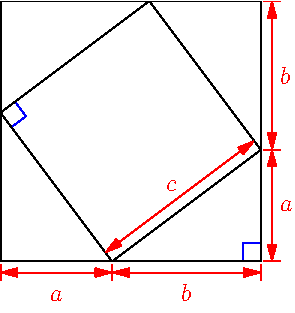
\includegraphics{pythagora.pdf}
\caption{畢氏定理圖解}
\label{fig:d1}
\end{figure}

\end{document}

